\documentclass[10pt,oneside,slovak,a4paper]{article}

\usepackage[slovak]{babel}
\usepackage[T1]{fontenc}
\usepackage[utf8]{inputenc}
\usepackage{graphicx}
\usepackage{url}
\usepackage{xcolor}
\usepackage{hyperref}
\usepackage{listings}
\usepackage{refstyle}
\usepackage[font={small,it}]{caption}
\usepackage{indentfirst}
%math and equations
\usepackage{mathtools}
\DeclarePairedDelimiter\ceil{\lceil}{\rceil}
\DeclarePairedDelimiter\floor{\lfloor}{\rfloor}

\usepackage{fancyhdr}
\pagestyle{fancy}
\fancyhf{}

%hlavicka dokumentu
\rhead{ID: 110867 }
\lhead{Matej Pakán}
%paticka dokumentu
\fancyfoot[CE,CO]{1. zadanie - SIP proxy - ústredňa}
\fancyfoot[LE,RO]{\thepage}

\usepackage{listings}
\usepackage{color}

\definecolor{mygreen}{rgb}{0,0.6,0}
\definecolor{mygray}{rgb}{0.5,0.5,0.5}
\definecolor{mymauve}{rgb}{0.58,0,0.82}

\lstdefinestyle{python}{
  belowcaptionskip=1\baselineskip,
  breaklines=true,
  frame=L,
  basicstyle=\tiny,
  xleftmargin=\parindent,
  language=C,
  showstringspaces=false,
  basicstyle=\footnotesize\ttfamily,
  keywordstyle=\bfseries\color{green!40!black},
  commentstyle=\itshape\color{purple!40!black},
  identifierstyle=\color{blue},
  stringstyle=\color{orange},
}

\lstdefinestyle{customasm}{
  belowcaptionskip=1\baselineskip,
  frame=L,
  xleftmargin=\parindent,
  language=[x86masm]Assembler,
  basicstyle=\footnotesize\ttfamily,
  commentstyle=\itshape\color{purple!40!black},
}

\lstset{escapechar=@,style=python}
%zdroj týchto nastavení': https://en.wikibooks.org/wiki/LaTeX/Source_Code_Listings     --upravené

\usepackage{cite}


\title{SIP Proxy - ústredňa\thanks{1. zadanie - SIP proxy – v predmete mobilné technológie a aplikácie, ak. rok 2021/22, cvičiaci: 
Ing. Matej Janeba}}

\author{Matej Pakán\\[2pt]
	{\small ID: 110867}\\
	{\small Slovenská technická univerzita v Bratislave}\\
	{\small Fakulta informatiky a informačných technológií}\\
	{\small \texttt{xpakan@stuba.sk}}
	}

\date{\small 1. marca 2022}



\begin{document}

\maketitle
\newpage
\tableofcontents{\protect\newpage}

\section{Znenie zadania}

\subsection{Hlavná myšlienka}
Na vašom počítači (alebo virtuálnom počítači) sprevádzkujte SIP Proxy, ktorá 
umožní prepájanie a realizáciu hovorov medzi štandardnými SIP klientami.

\subsection{Doplňujúce informácie k zadaniu}
Na implementáciu vašej SIP Proxy si môžete zvoliť \textbf{akýkoľvek} programovací jazyk a použiť \textbf{akúkoľvek} SIP 
knižnicu, ktorá pre daný programovací jazyk existuje. Vo výsledku však musíte spúšťať “váš kód”, v 
ktorom sú zakomponované knižnice, ktoré poskytujú funkcionalitu SIP Proxy. To znamená, že \textbf{nemôžete}
zobrať existujúcu SIP Proxy ako napr. Asterisk, kde len skompilujete alebo priamo spustíte cudziu 
binárku… Hovor \textbf{musí} byť realizovaný medzi dvomi \textbf{fyzickými} zariadeniami v rámci LAN siete.

\subsection{Rozsah povinných funkcionalít}
\begin{itemize}
\item{Registrácia účastníka (bez nutnosti autentifikácie)}
\item{Vytočenie hovoru a zvonenie na druhej strane}
\item{Prijatie hovoru druhou stranou, fungujúci hlasový hovor}
\item{Ukončenie hlasového hovoru (prijatého aj neprijatého)}
\end{itemize}
Ak sú splnené \textbf{všetky} tieto podmienky, študent získava 5 bodov, ktoré sú minimom na absolvovanie 
tohoto zadania.

\subsection{Doplnkové funkcionality}
\begin{itemize}
\item{Možnosť zrealizovať konferenčný hovor (aspoň 3 účastníci)}
\item{Možnosť presmerovať hovor}
\item{Možnosť realizovať videohovor}
\item{Logovanie “denníka hovorov” – kto kedy komu volal, kedy bol ktorý hovor prijatý, kedy bol ktorý 
hovor ukončený, do ľubovoľného textového súboru v ľubovoľnom formáte}
\item{Úprava SIP stavových kódov z zdrojovom kóde proxy, napr. “486 Busy Here” zmeníte na “486 
Obsadené”}
\end{itemize}

Každá doplnková funkcionalita predstavuje plus 1 bod.

Počas prezentácie zadania musíte byť schopní na zariadení, kde beží ústredňa urobiť SIP trace a otvoriť 
ho pomocou tcpdump alebo Wireshark, a v primeranom rozsahu vysvetliť cvičiacemu, ako daná 
signalizácia prebieha.

\section{Úvod}
Hneď od začiatku som vedel, že projekt budem chcieť realizovať v Pythone, kvôli najlepšiemu porozumeniu tohto jazyka a jednoduchým troubleshooting.
Ako knižnicu som použil \href{https://github.com/tirfil/PySipFullProxy/blob/master/sipfullproxy.py}{\underline{PySipFullProxy}} na odporúčanie vedúceho cvičení.
Ako SIP klienta som použil \href{https://www.linphone.org/}{\underline{Linphone}}, kvôli jednoduchému nastaveniu klientov.

\medskip
Verejný github repozitár k zdrojovému kódu a WireShark scenárom:

\href{https://github.com/Matt1s/MTAA-SIP-PROXY}{\underline{https://github.com/Matt1s/MTAA-SIP-PROXY}}

\section{Spúšťanie knižnice}
Knižnicu \href{https://github.com/tirfil/PySipFullProxy/blob/master/sipfullproxy.py}{\underline{PySipFullProxy}} bolo nutné upraviť, kvôli nekompatibilite s mojou verziou Pythonu (3.10).
Väčšinou išlo o chyby pri funkcii \textbf{join()} alebo pri \textbf{zakódovaní/dekódovaní z/do UTF-8}

Niekoľko riadkov som teda musel upraviť, napríklad:
\begin{lstlisting}
text = string.join(data,"\r\n")
\end{lstlisting}
na
\begin{lstlisting}
text = "\r\n".join(data)
\end{lstlisting}

a

\begin{lstlisting}
self.socket.sendto(text,self.client_address)
\end{lstlisting}
na
\begin{lstlisting}
self.socket.sendto(text.encode(),self.client_address)
\end{lstlisting}

a

\begin{lstlisting}
if registrar.has_key(origin):
\end{lstlisting}
na
\begin{lstlisting}
if origin in registrar:
\end{lstlisting}

Takisto som odstránil aj celú vetvu obsahujúcu rx\_invalid a rx\_invalid2, kvôli vypnutiu reštrikcií na správny beh servera.



Následne po odstránení všetkých chýb som spúštal svoj main.py s použitím knižnice tak, ako som uznal za vhodné.

Môj main.py:
\begin{lstlisting}
import sipfullproxy as SIP
import socket
def main():
    # moved these 2 variables as they are no longer needed in sipfullproxy.py file
    HOST = '0.0.0.0'
    PORT = 5060

    # edited filename
    SIP.logging.basicConfig(format='%(asctime)s:%(levelname)s:%(message)s',filename='zaznam.log',level=SIP.logging.INFO,datefmt='%H:%M:%S')
    SIP.logging.info(SIP.time.strftime("%a, %d %b %Y %H:%M:%S ", SIP.time.localtime()))

    #selecting specific IP address
    ipaddress = socket.gethostbyname_ex(socket.gethostname())[2][0]
    if ipaddress == "127.0.0.1":
        ipaddress = SIP.sys.argv[1]
    SIP.logging.info(ipaddress)
    SIP.recordroute = "Record-Route: <sip:%s:%d;lr>" % (ipaddress,PORT)
    SIP.topvia = "Via: SIP/2.0/UDP %s:%d" % (ipaddress,PORT)

    # setting up server
    server = SIP.socketserver.UDPServer((HOST, PORT), SIP.UDPHandler)
    try:
        print('Server starting at ' + ipaddress) 
        server.serve_forever()
    except:
        server.server_close()
        print('Server stopped, closing program...')
main()
\end{lstlisting}

V tomto riadku:
\begin{lstlisting}
ipaddress = socket.gethostbyname_ex(socket.gethostname())[2][0]
\end{lstlisting}
Vyberám zo zoznamu dostupným rozhraní, na ktorom konkrétnom rozhraní a s akou IP sa spustí môj SIP proxy server.

Následne pomocou \textbf{try/except} spúšťam server s informačnou správou, že kde je spustení. Pri násilnom vypnutí (CTRL+C) sa server vypne.

\newpage
\section{Scenáre - povinné funkcionality}

\subsection{Registrácia účastníka}

Analýza súboru '200 OK - registracia ucastnika.pcapng'- filter 'sip'
\begin{figure}[h]
\centerline{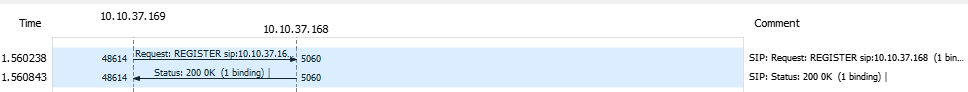
\includegraphics[scale=0.6]{./WireShark/FlowCharts/registracia.png}} 
\caption{Flow chart registrácia klienta}
\end{figure}

Žiadosť o registráciu sa snaží prejsť z '10.10.37.139' (môj mobil), ktorý už je na lokálnej sieti. Proxy server tohto používateľa zapíše a odpovie klientovi odpoveď STATUS: 200 OK, čo znamená, že klient bol úspešne zaregistrovaný. Keďže nerobíme autorizáciu klientov, tak tam nič nechýba. Ak by sme autorizáciu robili, potrebovali by sme ešte jeden REGISTER a odpoveď 401 Unauthorized s registračnými údajmi. Ústredňa teda používateľa registruje napriamo bez autorizácie.V message header správy REGISTER je 'to' a 'from' rovnaké.

\subsection{Vytočenie hovoru a zvonenie na druhej strane}
Analýza súboru '100 trying 180 ringing - vytocenie a zvonenie.pcapng' - filter 'sip'
\begin{figure}[h]
\centerline{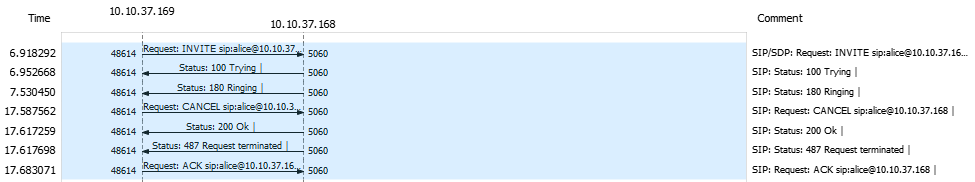
\includegraphics[scale=0.6]{./WireShark/FlowCharts/tryingandringing.png}} 
\caption{Flow chart vytočenie a zvonenie klienta}
\end{figure}

Po úspešnej registrácii zo strany mobilu s IP '10.10.37.139' odchádza INVITE pre 'alice@10.10.37.168'. Z ústredne následne prichádza odpoveď 100 Trying a 180 Ringing. Teda na druhej strane (Alice) začína zvoniť.
Po pár sekundách Bob zruší hovor kliknutím na tlačidlo skončiť, teda prechádza Request CANCEL, odpoveď 200 OK a teda hovor bol zrušený zo strany Boba (volajúci).  

\newpage

\subsection{Prijatie hovoru druhou stranou, fungujúci hlasový hovor}
Analýza súboru '200 OK - hlasovy hovor.pcapng' - filter 'sip'
\begin{figure}[h]
\centerline{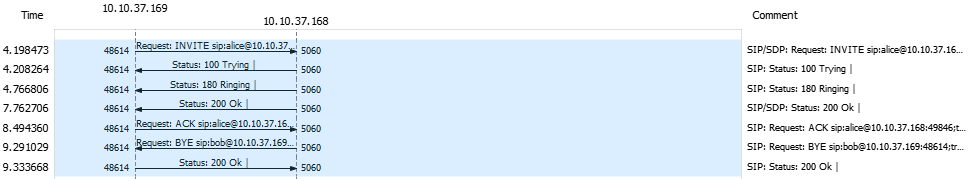
\includegraphics[scale=0.6]{./WireShark/FlowCharts/hlasovyhovor.png}} 
\caption{Flow chart hlasový hovor}
\end{figure}
Hlasový hovor prebieha po prijatí druhou stranou (Bob volá Alice). Následne 2 sekundy prebieha hovor cez SIP/SDP protokol. V invite správe si môžeme pozrieť ponúknuté kodeky, ktoré ak druha strana spustí, budú medzi sebou správne komunikovať. V INVITE takisto oznamuje, na akom porte bude daný klient počúvať.

\medskip

Pri aplikovaní filtra 'sip || rtp' je možné si zobraziť aj tok hlasových dát a informácie o tom, aké kodeky boli použité.

\newpage

\subsection{Ukončenie hlasového hovoru (prijatého aj neprijatého)}

Analýza súboru '200 OK - hlasovy hovor.pcapng' - filter 'sip'
\begin{figure}[h]
\centerline{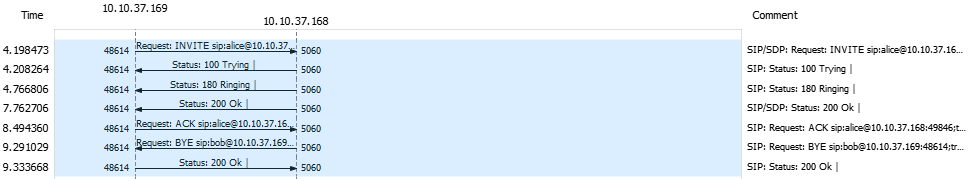
\includegraphics[scale=0.6]{./WireShark/FlowCharts/hlasovyhovor.png}} 
\caption{Flow chart hlasový hovor (rovnaký obr. ako vyššie)}
\end{figure}

Na konci flowu vidíme BYE a ACK, teda signalizačné správy o tom, že nadviazaný hovor je ukončený a druhá strana je s tým oboznámená.

\medskip

Analýza súboru '486 Busy here - neprijaty hovor.pcapng' - filter 'sip'
\begin{figure}[h]
\centerline{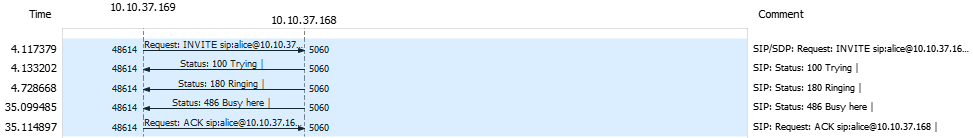
\includegraphics[scale=0.6]{./WireShark/FlowCharts/busyhere.png}} 
\caption{Flow chart 486 Busy here}
\end{figure}

Podobný scenár ako v sekcii 'Vytočenie hovoru a zvonenie na druhej strane', akurát ústredňa vracia po 30 sekundách 486 Busy here, teda Bob vytočil Alice, ale tá nestihla zdvihnúť do doby 30 sekúnd. Hovoríme teda o neprijatom hovore.

\medskip

Analýza súboru '603 Decline - odmietnutie hovoru.pcapng' - filter 'sip'
\begin{figure}[h]
\centerline{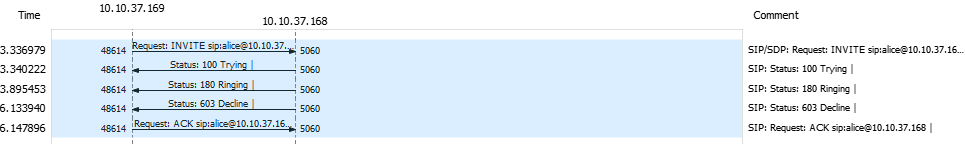
\includegraphics[scale=0.6]{./WireShark/FlowCharts/decline.png}} 
\caption{Flow chart 603 Decline}
\end{figure}

Rovnaký scenár ako vyššie, miesto nezdvihnutia (ignorovania) ale Alice zrušila (odmietla) hovor, preto Bob dostal informáciu z ústredne 603 Decline.

\newpage
\section{Scenáre - doplnkové funkcionality}
\subsection{Realizácia konferenčného hovoru (aspoň 3 účastníci)}
Analýza súboru 'KONFERENCNY HOVOR.pcapng' - filter 'sip'
\begin{figure}[h]
\centerline{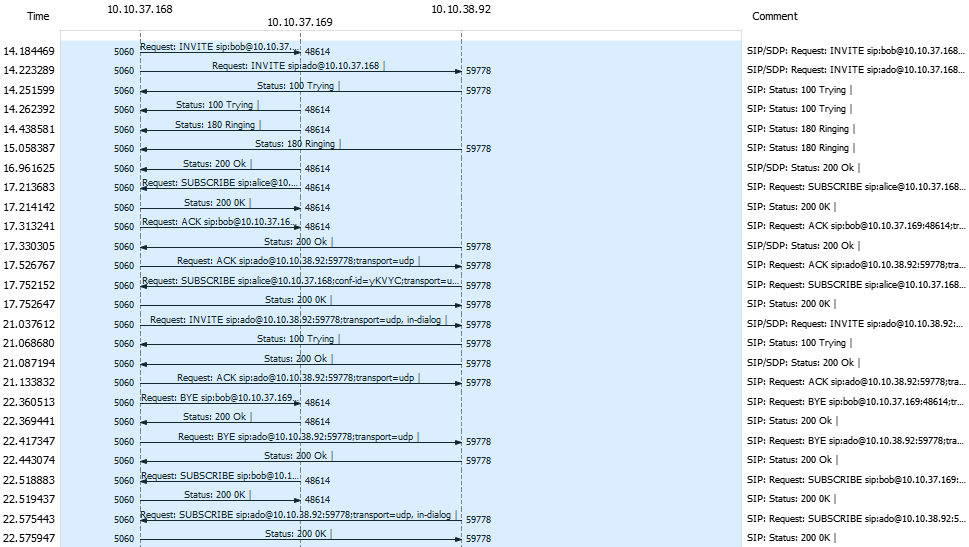
\includegraphics[scale=0.6]{./WireShark/FlowCharts/konferencnyhovor.png}} 
\caption{Flow chart konferenčný hovor (3 ľudia)}
\end{figure}

Pozvánka na konferenčný išla od užívateľa Alice užívateľom Bob a Ado. Na obrázku preto vidíme 2x 100 Trying a 180 Ringing. Odpovede 200 OK nasvedčujú tomu, že všetko prebieha v poriadku a hovor sa spustil medzi 3 ľudmi.  Následne vidíme novú správu SUBSCRIBE o tom, že volajúci chce byť informovaný ak sa ďalší účastník pripojí do hovoru.
Neskôr zase vidíme správu BYE od používateľa Ado. To znamená, že hovor pokračuje už len medzi 2 ľudmi. 

\newpage 

\subsection{Presmerovanie hovoru}
Analýza súboru 'PRESMEROVANIE.pcapng' - filter 'sip'
\begin{figure}[h]
\centerline{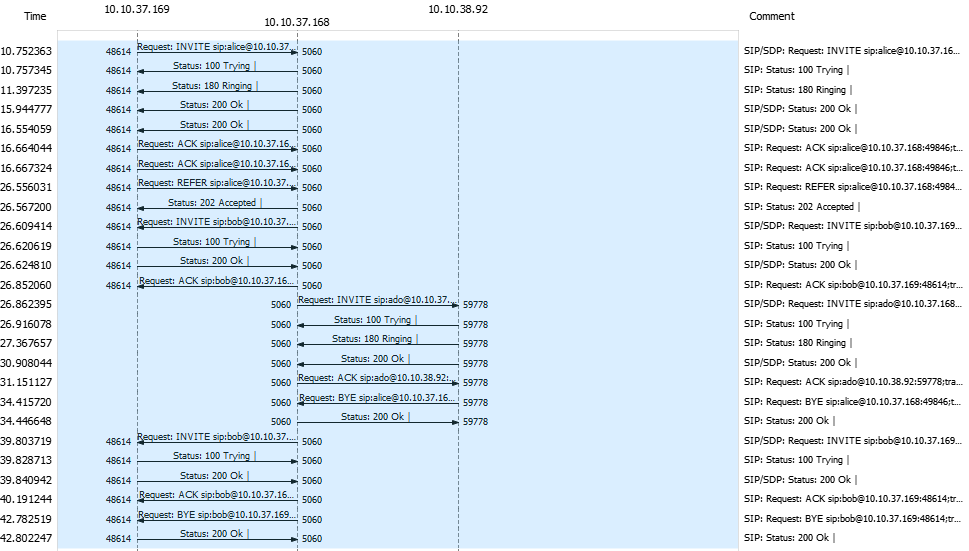
\includegraphics[scale=0.6]{./WireShark/FlowCharts/presmerovanie.png}} 
\caption{Flow chart presmerovanie}
\end{figure}

Na obrázku vidíme, ako bola nadviazaná komunikácia medzi Bobom (10.10.37.169) a Alice (10.10.37.168). Následne Bob presmeroval hovor na Ado (10.10.37.92), tým pádom hovor prebiehal iba medzi Alice a Ado (u Boba hrá hudba). Potom Ado hovor zrušil (BYE a ACK) a hovor sa vrátil do normálu medzi Bob a Alice. Nakonci prebieha štandardné ukončenie hovoru pomocou BYE a ACK.

\newpage

\subsection{Realizácia videohovoru}
Analýza súboru 'VIDEOHOVOR.pcapng' - filter 'sip'
\begin{figure}[h]
\centerline{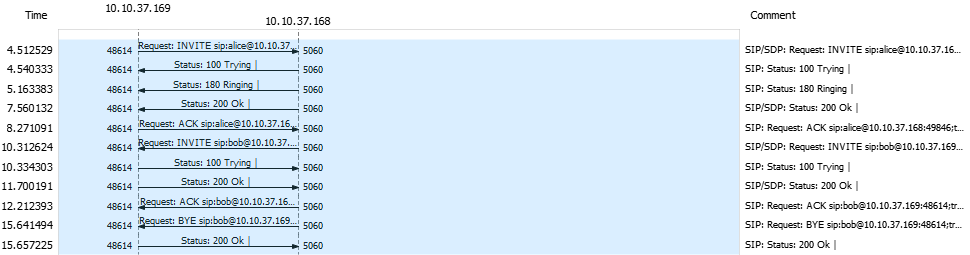
\includegraphics[scale=0.6]{./WireShark/FlowCharts/videohovor.png}} 
\caption{Flow chart videohovor}
\end{figure}

Rozdiel oproti štandardnému hlasovému hovoru je v tom, že po nadviazaní hlasového hovoru ide ešte jeden INVITE, 100 Trying a 200 OK (žiadosť o zapnutie kamery).
Hovor sa inak líši iba v použitých kodekoch. Nakonci záznamu je štandardné ukončenie hovoru pomocou BYE a ACK.

\section{Záver}
Čakal som že bude zložitejšie rozbehať vlastný proxy server na realizáciu hovor, za použitia knižnice to bolo omnoho jednoduchšie.
Pomocou WireSharku bolo pekne vidieť ako sa všetky packety presúvajú. Bol pekný pocit keď sa podarilo rozbehnúť videohovor :)

\medskip
Verejný github repozitár k zdrojovému kódu a WireShark scenárom:

\href{https://github.com/Matt1s/MTAA-SIP-PROXY}{\underline{https://github.com/Matt1s/MTAA-SIP-PROXY}}

\end{document}



























